 \chapter{\label{ch5-calibration}Calibration} 

\minitoc

\notes[inline,caption={}]{
	\section{Plan}
	\subsection{Topics}
	\begin{itemize}
		\item Pedestal subtraction
		\item Transfer functions
		\item Gain Matching
		\item SPE
		\item Flat fielding
		\item Time correction
		\item Future
		\begin{itemize}
			\item Live calibration
		\end{itemize}
	\end{itemize}
	\subsection{Questions}
	\begin{itemize}
		\item TARGET architecture diagram, Wilkinson ADC 
		\item How much detail about all the TF approaches do I go into?
	\end{itemize}
}


\change[inline]{Flow diagrams? See Cyril talk 18/07/06 camera calibration call}

\lstset{language=Python}

\section{Introduction}

In order to obtain meaningful and reliable results from the camera, a number of calibrations must be applied to the waveforms read. A primary objective of my DPhil was to investigate the most optimal and efficient approaches for these calibrations (in accordance with the \gls{cta} requirements described in Chapter~\ref{ch3-architecture}), and to determine if additional calibrations are required.

When I joined the \gls{chec} development, the calibration discussion was still in its infancy. Some approaches had been tested in a laboratory environment \cite{Bechtol2012}, but there had been little discussion on how exactly the calibrations could be applied efficiently in an analysis pipeline, where one might not be able to use the same detailed calibration due to limited resources (such as memory and processing time). A major contribution of my DPhil was to prototype the calibration procedures, develop an approach for a calibration pipeline, write the software to perform such a pipeline, and finally assess its performance. This was an iterative process, the development of which is still ongoing. However, a procedure now exists that allows us to obtain meaningful results from the waveform data, a capability that is of paramount importance in the commissioning of the camera.

In this chapter I will outline each of the calibration steps that are presently adopted for \gls{chec}. They are introduced in the general order that they are applied, and split into the categories of \gls{target} \gls{asic}, photosensor, and "other" calibrations.

\section{TARGET Calibration}

The calibrations described in this section relate to the \gls{target} module. As detailed in Chapter~\ref{ch2-mechanics}, the \gls{target} \gls{asic} is responsible for the sampling, digitisation and readout of the waveform data. As a result, there are two calibrations that are solely related to the \gls{target} \gls{asic}: electronic pedestal subtraction and the linearity correction via the transfer function. 

The functional block diagram of the \gls{target} \gls{asic} in Figure~\ref{fig:target5diagram} outlines the electronics that require calibration, and can be used as a reference in the following descriptions.

As the calibrations in this section are very low-level, and related to \gls{chec}'s specific \gls{fee}, they are handled by the TargetCalib library (Chapter~\ref{ch4-software}).

\subsection{Electronic Pedestal Subtraction}

\begin{figure}
\begin{minipage}[t]{.49\textwidth}
  \centering
  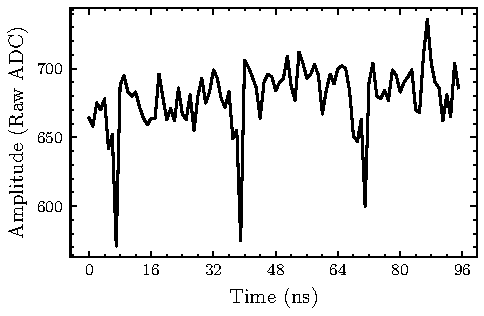
\includegraphics[width=0.92\textwidth]{rawwf_10} 
  \captionof{figure}[Raw waveform]{TARGET-C waveform as read out from CHEC-S, showing the electronic pedestal in the absence of any other input, before any calibration is applied.}
  \label{fig:rawwf}
\end{minipage}%
\hfill
\begin{minipage}[t]{.49\textwidth}
  \centering
  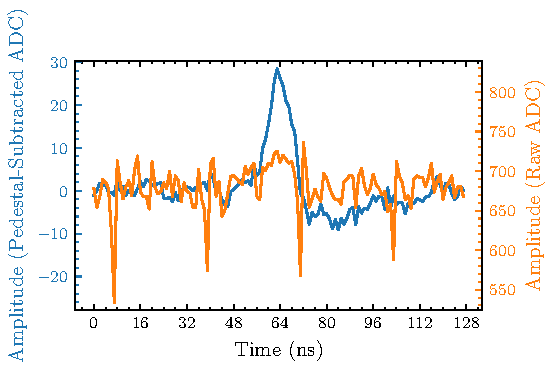
\includegraphics[width=\textwidth]{pulse_raw_vs_pedestal}
  \captionof{figure}[Comparison of pedestal-subtracted waveform with raw waveform]{CHEC-S waveform  containing a \SI{5}{\pe} pulse, before and after pedestal subtraction.}
  \label{fig:pulse_raw_vs_pedestal}
\end{minipage}
\end{figure}

\begin{figure}
  \begin{subfigure}[b]{0.49\textwidth}
    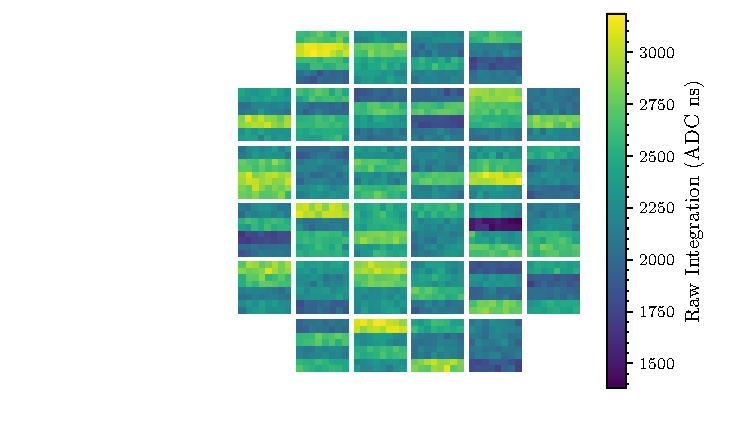
\includegraphics[width=\textwidth]{r0_cherenkov_image_mirrored_cropped}
    \caption{Raw image.}
    \label{fig:r0_cherenkov_image_mirrored_cropped}
  \end{subfigure}
  \hfill
  \begin{subfigure}[b]{0.49\textwidth}
    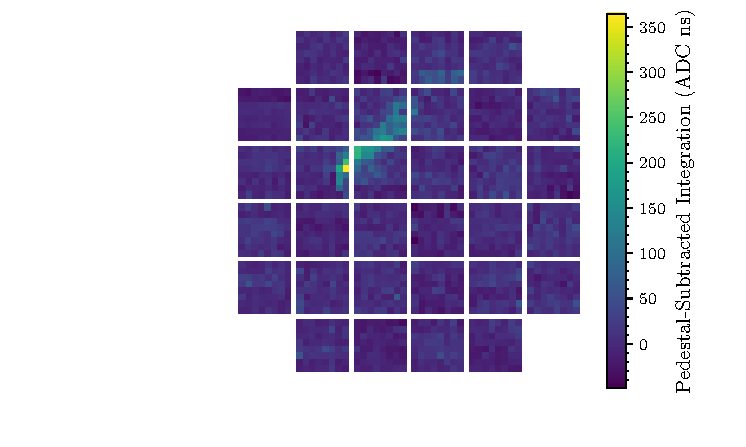
\includegraphics[width=\textwidth]{r1_cherenkov_image_mirrored_cropped}
    \caption{Pedestal-subtracted image.}
    \label{fig:r1_cherenkov_image_mirrored_cropped}
  \end{subfigure}
  \centering
  \begin{subfigure}[b]{0.49\textwidth}
    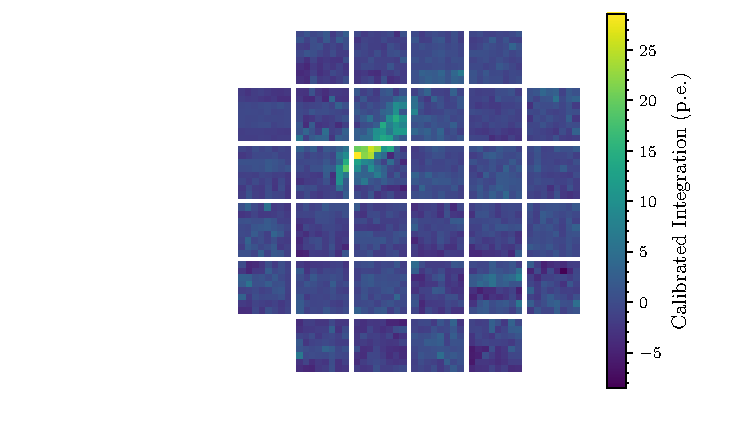
\includegraphics[width=\textwidth]{r1pe_cherenkov_image_mirrored_cropped}
    \caption{Final calibrated image.}
    \label{fig:r1pe_cherenkov_image_mirrored_cropped}
  \end{subfigure}
  \caption[Comparison of calibration stages with a Cherenkov shower image.]{The same image of a Cherenkov shower taken with CHEC-M, but at different stages of calibration. An integration window was chosen using the \textit{Neighbour Peak Finding} technique (Chapter~\ref{ch6-reduction}) on the \si{\pe} calibrated waveforms. The same samples were then integrated for each of the calibration stages.}
\end{figure}

The most important, but also the simplest, calibration to apply ti the waveform data is the subtraction of the electronic pedestal. Each cell in the storage array of the \gls{asic} is a unique capacitor. For a specific \gls{vped}, each capacitor has its own resulting electronic pedestal value. As each sample of the waveform corresponds to a single storage cell, each sample therefore has a unique pedestal value to be subtracted. This is apparent in Figures~\ref{fig:rawwf}~and~\ref{fig:pulse_raw_vs_pedestal} where the variation from sample-to-sample is very large in the raw waveform, and the low-amplitude pulses are almost indistinguishable. The fluctuations in the raw waveforms between pixels is also significant, to the point where low-amplitude Cherenkov showers are undetectable in the camera (Figure~\ref{fig:r0_cherenkov_image_mirrored_cropped}). However, the dominating variations are between \glspl{asic}. As a result, the outlines of the \glspl{asic} are the dominating feature in camera images containing raw samples, such as Figure~\ref{fig:r0_cherenkov_image_mirrored_cropped}. With a pedestal-subtraction calibration alone, the waveforms are transformed into a state in which a moderate amount of Cherenkov shower assessment can be performed, as demonstrated in Figure~\ref{fig:r1_cherenkov_image_mirrored_cropped}.

\begin{figure}
	\centering
    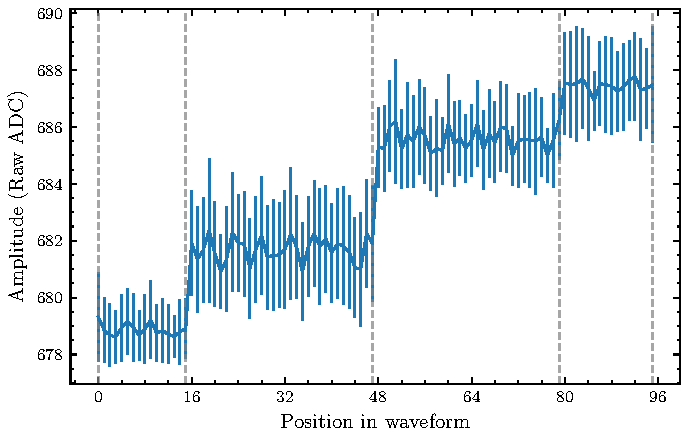
\includegraphics[width=\textwidth]{cellwf_15} 
	\caption[Storage-cell-amplitude dependence on position in the waveform.]{Average amplitude of the electronic pedestal for a single storage cell in a TARGET-C ASIC, at different positions in the waveform. Error bars indicate the standard deviation of the amplitudes. The grey dashed lines indicate the position of the block edges in the waveform for this cell. The average of the values inside each block segment equals the pedestal value stored in the lookup table for that cell, in each of those block positions.} 
	\label{fig:cellwf}
\end{figure}

There are $2^{14} = 16,384$ storage cells per channel (for \gls{chec-m}, $2^{12} = 4096$ for \gls{chec-s}\otherch{Make sure to mention about the difference in number of cells for checs in ch2}), therefore one could naively conclude that there are $32 (Modules) * 64 (Channels) * 16,384 (Cells)$ pedestal values to keep record of. However, an additional characteristic of the \gls{target} \gls{asic} is that the pedestal amplitude depends on the position in the waveform. The source of this characteristic is due to the fact that the storage cell blocks are not entirely decoupled from each other; the discharge of one block affects adjacent blocks. This effect is apparent in Figure~\ref{fig:cellwf}, where the pedestal amplitude of a single cell changes depending on the position of its parent block in the waveform. Consequently, an extra dimension of ``position in waveform'' must be considered in the waveform lookup table.

\subsubsection{Generation}

In order to perform the pedestal subtraction, one must first generate a lookup table of pedestal values. This can be easily obtained with a calibration run where the voltages across the photosensor are disabled, and forcing the camera to trigger (with either an external pulse generator, or internally via software) to obtain a large amount of waveform data. Typically around 30,000 events provide enough samples for every storage cell, in every waveform position, to have at least 10 entries. The samples are then collected as a running average with the dimensions $[Module, Channel, Starting Block, Blockphase+Sample\_i]$, where the $Starting Block$ is the storage block that the first sample in the waveform belongs to, $Blockphase$ is the cell index within the storage block that the waveform begins on, and $Sample\_i$ is the index of each sample in the waveform. This is illustrated in Figure~\change{include figure, and edit to use bp 8 and 12}, where for these two readout windows shown, the pedestal running average |Pedestal[TM][CHANNEL][9][8:103]| and |Pedestal[TM][CHANNEL][8][12:107]| will be contributed to, respectively.

The TargetCalib library handles the pedestal lookup table generation, and stores it into a \gls{fits} file. A new pedestal file is typically generated at the start of each new dataset, as the dependencies on temperature and evolution with time are still being investigated.

\subsubsection{Application}

To apply the pedestal, the entry within the lookup table that corresponds to each sample is subtracted from the waveform. The result of the subtraction can be seen in Figures~\ref{fig:pulse_raw_vs_pedestal}~and~\ref{fig:r1_cherenkov_image_mirrored_cropped}. 

\subsubsection{Performance}

\begin{figure}
	\centering
    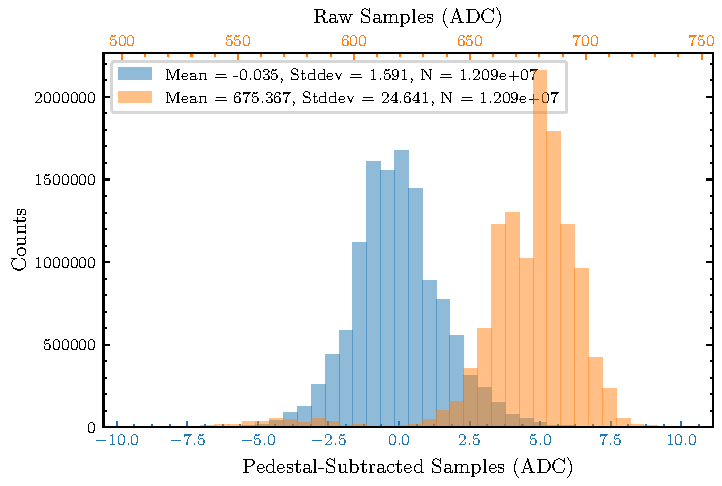
\includegraphics[width=\textwidth]{pedestal_hist} 
	\caption[Spread of electronic-pedestal values before and after the pedestal subtraction.]{Spread of electronic-pedestal values before and after the pedestal subtraction for a single TARGET-C channel. The waveforms used to create the pedestal lookup table are separate to those used in these histograms.} 
	\label{fig:pedestalresiduals}
\end{figure}

The primary quantification of this calibration's performance is the standard deviation of electronic-pedestal samples that have had separately-created pedestal values subtracted from them. Figure~\ref{fig:pedestalresiduals} demonstrates the performance of the pedestal subtraction for a \gls{targetc} channel, achieving a residual variation of \SI{1.6}{ADC} (approximately \SI{0.5}{\pe})\final{update value}.

\subsection{Transfer Function}

The other calibration related to the digitisation and readout inside the \gls{target} \gls{asic} is caused by the non-linearities in the storing and reading of charge to and from the storage cells. The components responsible for the need for this calibration are the sampling array, gain/buffer amps, and the Wilkinson \glspl{adc}, seen in Figure~\ref{fig:target5diagram}. The non-linearity of these components is propagated to the sample readout - a sample with twice the amplitude input into \gls{target} will have less than twice the amplitude when readout.

To correct for this non-linearity, a look-up table is generated to convert from the sample amplitude that is read out from the \gls{asic} (in \si{ADC}) to the sample amplitude that is input into the \gls{asic} (in \si{mV}). This look-up table is known as the Transfer Function. As one might expect, each sampling cell has its own linear response to account for, and therefore a look-up table is typically required at least per channel and per sampling cell, however a noticeably improved performance is observed by considering a Transfer Function per storage cell \otherch{need to show this, maybe in TF Investigations appendix?}.

There are two forms of Transfer Function that have been considered for \gls{chec}, distinguished by the type of input used to generate them. A \gls{dc} Transfer Function is created by applying a constant \gls{dc} input of known voltage into the module, and iterating over the full dynamic range by varying the voltage. An \gls{ac} Transfer Function is generated by inputting a pulse of a known amplitude with a shape expected from the photosensor, and iterating as with the \gls{dc} approach. During previous investigations of the \gls{target} module, where sinusoidal signals were input into the module, a dependence on the signal frequency and input amplitude was observed that acts to further reduce the output amplitude \cite{Bechtol2012}\cite{Albert2017}. The source of this dependence was deemed to be due to the amplifiers, which cannot slew fast enough to keep up with the input signal if the frequency and amplitude are large. Due to the use of a pulse to generate the \gls{ac} Transfer Functions, the result inherently includes the correction required for the frequency that the pulses correspond to. 

\begin{figure}
  \begin{subfigure}[b]{0.49\textwidth}
    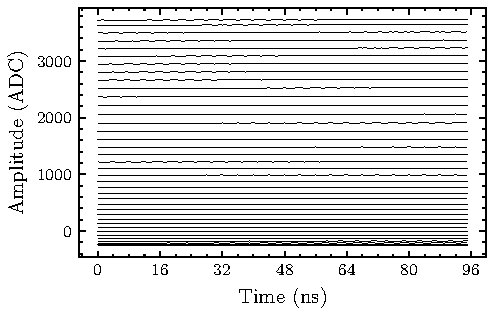
\includegraphics[width=\textwidth]{generation_t5}
    \caption{DC Transfer Function input, measured with TARGET~5.}
    \label{fig:generation_t5}
  \end{subfigure}
  \hfill
  \begin{subfigure}[b]{0.49\textwidth}
    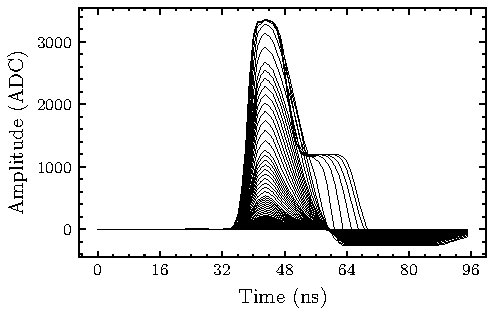
\includegraphics[width=\textwidth]{generation_tc}
    \caption{AC Transfer Function input, measured with TARGET~C.}
    \label{fig:generation_tc}
  \end{subfigure}
  \caption[Transfer Function generation waveforms.]{Multiple average waveforms, increasing in amplitude. Each average contains 1000 waveforms from the same single channel. These waveforms cover the full dynamic range of the TARGET ASIC, and are used as inputs to generate the DC and AC Transfer Functions, respectively. The saturation behaviour of the TARGET C ASIC can be seen in the high amplitude waveforms in (b).}
\end{figure}

\begin{figure}
  \begin{subfigure}[b]{0.49\textwidth}
    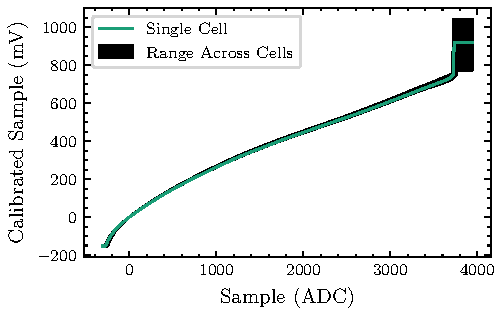
\includegraphics[width=\textwidth]{lookup_t5}
    \caption{DC Transfer Function lookup table, measured with TARGET~5. Contains 64 Transfer Functions, one for each Sampling Cell.}
    \label{fig:lookup_t5}
  \end{subfigure}
  \hfill
  \begin{subfigure}[b]{0.49\textwidth}
    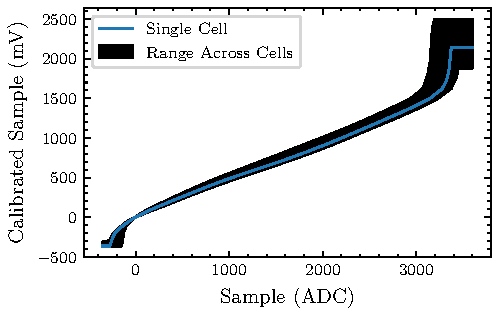
\includegraphics[width=\textwidth]{lookup_tc}
    \caption{AC Transfer Function lookup table, measured with TARGET~C. Contains 4,096 Transfer Functions, one for each Storage Cell.}
    \label{fig:lookup_tc}
  \end{subfigure}
  \caption[Transfer Function lookup tables.]{The Transfer Function lookup tables for a single channel.}
\end{figure}

\subsubsection{Generation (\gls{dc} Transfer Function)}

During the commissioning of \gls{chec-m}, a \gls{dc} Transfer Function was used with no \gls{ac} corrections. To generate this Transfer Function, the internal input pedestal voltage (Vped) setting is used to apply a \gls{dc} voltage offset of known amplitude. By repeating the process for Vped values from \SI{500}{mV} to \SI{1700}{mV}, in steps of \SI{25}{mV}, the full dynamic range of the module is explored, covering the range \SI{-250}{ADC} to \SI{3700}{ADC} (Figure~\ref{generation_t5}). The running averages of the ADC samples are grouped and monitored according to $[Module, Channel, Sampling~Cell, Input~Amplitude]$, utilising every sample in the waveform. Around 1,000 events are required to provide sufficient statistics.

The second step in the generation of the \gls{dc} Transfer Function is to linearly interpolate the running averages at the ADC points defined by the user. This provides a lookup table of \si{mV} values with dimensions $[Module, Channel, Sampling~Cell, ADC~Value]$ that can be used to provide a calibrated value for a measured ADC value. The lookup table for a single channel is illustrated in Figure~\ref{fig:lookup_t5}. This table is saved to a \gls{fits} file, ready for application. A fresh \gls{dc} Transfer Function lookup table was typically created once a day during the \gls{chec-m} commissioning.

\subsubsection{Generation (\gls{ac} Transfer Function)}

\begin{figure}
	\centering
    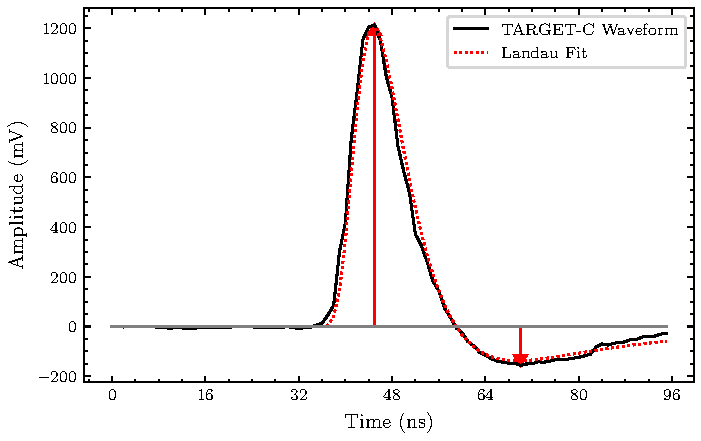
\includegraphics[width=\textwidth]{tf_pulse_fit} 
	\caption[Fit of the waveform in order to extract samples to generate the AC Transfer Function.]{An example of the amplitude extraction used for generating the AC Transfer Function. The waveform is fit with two Landau functions (red curve). The samples of the waveform that occur at the time of the minimum and maximum of the fit (red arrows) are used as the inputs to the AC Transfer Function.} 
	\label{fig:tf_pulse_fit}
\end{figure}

As the ability to internally set a \gls{dc} voltage with a known amplitude via the Vped was removed in \gls{targetc} (see \ref{ch2-mechanics}) \otherch{more precise ref, and remember to mention this change}, and the ability to input a \gls{dc} voltage externally is prohibited by the \gls{ac} coupling of the module \otherch{remember to introduce ac coupling}, the decision was made to transition to an \gls{ac} Transfer Function that uses the expected pulse shape as an input. This approach therefore corrects for the \gls{ac} effect with the appropriate frequency. However, in order to externally input pulses from a pulse generator the module must be removed from the camera. Therefore, the \gls{ac} Transfer Function is only generated once in the present calibration pipeline.
	
The full dynamic range is once again probed, by injecting pulses of varying amplitude. In order to extract the values that correspond to negative amplitudes in this method, the amplitude of the input undershoot is also monitored. Only the samples that correspond to the maximum of the input pulse (and minimum of the undershoot) has a ``true'' amplitude of the input amplitude. Therefore, to extract the correct samples, each waveform is fitted with two Landau functions, a fair approximation to the pulse shape (Figure~\change{figure showing the fit}). Consequently, only two samples are extracted per waveform, requiring a much larger population of events (\utilde200,000) in order to generate a reliable running average grouped according to $[Module, Channel, Storage Cell, Input Amplitude]$. It is important to note that a Transfer Function per storage cell was adopted for \gls{targetc}, as it was found to significantly improve the residuals (see Appendix~\ref{a1-tf} for further discussion).

The second step in the generation of the \gls{ac} Transfer Function is identical to that in the \gls{dc} case. The resulting lookup table for a single channel can be seen in Figure~\ref{fig:lookup_tc}.

\subsubsection{Application}

Irrespective of the Transfer Function type, the lookup tables are stored in a format which enables them to be applied identically. When calibrating an ADC sample, the relevant lookup table is obtained according to the channel and cell of the sample, and is linearly interpolated to provide the calibrated \si{mV} value for the specified ADC value.

\subsubsection{Performance}

Due to its complexity and variety of approaches, the Transfer Function is still one of the most actively discussed aspects of the \gls{chec} calibration, and holds the highest potential for improvements among the different calibrations. Some possibilities for improvement include:
\begin{itemize}
	\item An improved sample extraction method for the \gls{ac} Transfer Function Waveform,
	\item The possibility for a \gls{dc} approach for \gls{targetc},
	\item Returning to the approach described in earlier \gls{target} studies where the pedestal is included inside the Transfer Function \cite{Albert2017},
	\item Alternatives to linear interpolation, such as Piecewise Cubic Hermite Interpolating Polynomial (PCHIP),
	\item Exchanging the lookup table for a parametrised regression characterisation of the Transfer Function (such as a high-order polynomial),
	\item Deciding between "per storage cell" or "per sampling cell",
	\item Inclusion of temperature corrections.
\end{itemize}
Appendix~\ref{a1-tf} provides some insight into the current progression in these active investigations.

Assessing the performance of the Transfer Functions is a more complicated task than for the pedestals. We are no longer comparing to a null signal, and instead comparing to an input amplitude which contains its own uncertainty, and could potentially be incorrect. So while the performance results may indicate that the residuals of the Transfer Function are small, this does not necessarily mean the calibration is accurate. Therefore, the most decisive performance indicator should be one that provides an independent measurement on the ``correct'' amplitude. The most obvious scheme fitting this requirement is the charge resolution, described in Chapter~\ref{ch3-architecture}, the results of which are explored in Appendix~\ref{a1-tf}.

\section{Photosensor Calibration} \label{section:photosensor_calib}

The other primary component in the detector chain that requires calibration is the photosensor itself. As photosensors are a much more common instrument used in a variety of experiments, the calibration procedures required are already well known in the academic community. It is therefore mostly a simple case of adapting existing approaches to fit our requirements.

The typical procedure in Cherenkov camera waveform analysis includes extracting the signal charge from the waveform of each pixel. This procedure, and the different methods to achieve it, is described in Chapter~\ref{ch6-reduction}. The value extracted is typically in digitisation counts or units of voltage, multiplied by time if the charge extraction approach is an integral over the waveform. For example, the units of the extracted charge from \gls{chec-s} using the \textit{Cross-Correlation} method (see Section~\ref{section:crosscorrelation}) is \si{mV ns}. Once extracted, this charge must be corrected for the relative efficiency of its pixel compared to the mean of the camera in order to achieve a uniform response (``flat-fielding''), and then converted into a counting unit that is common among the telescopes in the array (such as photons or photoelectrons), thereby simplifying the processing of array data \cite{Aharonian2004}. This procedure is characterised in the equation: 
\begin{equation} \label{eq:photosensor_calibration}
I_i = \frac{{A_Q}_i - {A_0}_i}{\gamma_{Q}} \times {\gamma_{FF}}_i,
\end{equation}
where 
\begin{itemize}
\item ${A_Q}_i$ is the charge extracted in units of \si{mV ns} for pixel $i$, proportional to the number of photoelectrons,
\item ${A_0}_i$ is the baseline in the absence of a signal for pixel $i$. It should be obtained using the same charge extraction approach used for the signal,
\item $\gamma_{Q}$ is the nominal conversion value from \si{mV ns} to photoelectrons/photons for the entire camera,
\item ${\gamma_{FF}}_i$ is the flat-field coefficient for the pixel $i$,
\item and $I_i$ is the resulting calibrated signal in photoelectrons/photons.
\end{itemize}

In the final calibration design of \gls{cta}, ${A_0}_i$ is intended to be supplied by the telescope alongside the waveforms at regular intervals. The regular updating of this value ensures that any changes to the baseline due to \gls{nsb} or temperature variations (which can also increase \gls{dcr}) are accounted for. However, this parameter was set to zero for the content of this thesis, and was not investigated. Instead, a less effective but simpler baseline subtraction was performed by monitoring the running average of the first 16 samples of the past 50 waveforms for each pixel. This running average was subtracted from each waveform before charge extraction. The remainder of this section will describe how to obtain the other calibration values, $\gamma_{Q}$ and ${\gamma_{FF}}_i$, and the other procedures related to the photosensor calibration.

\subsection{Gain Matching}

\begin{figure}
	\centering
    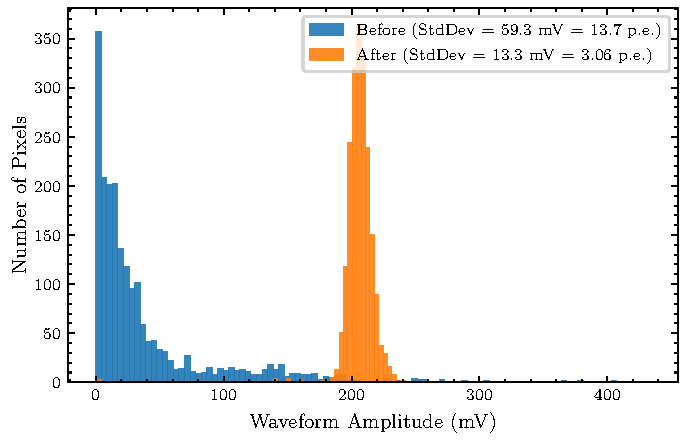
\includegraphics[width=\textwidth]{before_after_gm} 
	\caption[Gain-Matching Residuals]{Comparison between the spread in the average signal amplitude per pixel before and after gain matching, for a dataset with approximately \SI{50}{\pe} average illumination. Every pixel in the camera was included.} 
	\label{fig:before_after_gm}
\end{figure}

The flat-field coefficients, ${\gamma_{FF}}_i$, provide an offline compensation for a variety of photosensor parameters which alter the signal response in the waveform, described in Tables~x\&y\change{create table in mechanics chapter that list each parameter for the photosensor, with descriptions and specify if it changes with voltage, temperature, and how it affects signal}. However, as seen in the table, many of these parameters have a dependence on the voltages across the photosensor, which is a controllable value. With the \gls{chec-m} \glspl{mapmt} it is only possible to change the voltage value for an entire module, whereas with the \gls{chec-s} \glspl{sipmt} the voltages can be configured per superpixel (group of four pixels)\change{mention superpixels in ch3}. Therefore, voltage values can be selected before data-taking which result in a more uniform signal response across the photosensor. This is referred as ``Gain Matching'', however the name is slightly misleading, as it is the signal that is being matched, not the gain. It is performed by specifying the amplitude (in \si{mV}) that every pixel should be matched to, and then performing the following iterative procedure:
\begin{enumerate}
	\item The camera is uniformly illuminated with approximately \SI{50}{\pe}.
	\item The waveforms are readout, calibrated, and averaged per superpixel/module (excluding any dead pixels).
    \item The peak amplitudes of the average waveforms are extracted.
    \item Each module/superpixel is categorised as being above or below the requested amplitude.
    \item Depending on their category, the voltage setting is increased or reduced by steps of 5 (in units of DAC value), such that it increments closer to the requested amplitude. If the amplitude has been overstepped in the previous measurement, a smaller step value is used. The minimum DAC step value available is 1, which corresponds to $\frac{10}{256}$~V. If the amplitude is not responding to changes in voltage, the pixel is classified as ``dead'', and excluded from the average waveforms.
    \item The new voltage settings are applied and the process is repeated.
\end{enumerate}

In the future, this iterative technique will be replaced with a set of lookup tables for different requested amplitudes. These lookup tables will contain the final voltage settings resulting from this iterative technique. Additionally in the future, the requested signal will not be specified in terms of peak amplitude, but in terms of the \textit{Cross Correlation} charge extraction approach. The improvement in signal response for \gls{chec-s} as a result of the gain matching is shown in Figure~\ref{fig:before_after_gm}, where a response spread reduction of 22\% is achieved.

Tables~x\&y\change{update} also show a dependence on temperature for some of the photosensor parameters. The additional benefit of the gain matching is that temperature dependences can also be accounted for, by using the monitored temperature value per module and a lookup table of the appropriate corrections to the voltages, such that a constant signal response is kept across the camera. This particular in-situ calibration has not yet been implemented, but is intended for the future.

\change[inline]{plot with gain vs temperature? maybe some initial results from Yuki}

\subsection{SPE Fitting}

Due to the photon-counting nature of \glspl{mapmt} and \glspl{sipmt}, when the signal extracted from a pixel, illuminated with a low light-level (\utilde\SI{1}{\pe}), is accumulated into a histogram, the resulting spectra (Figure~\change{figure of both checm and checs spectra}) show peaks at regular intervals corresponding to the baseline (zeroth peak), \SI{1}{\pe} (first peak), \SI{2}{\pe} (second peak), etc. These spectra are referred to as ``\gls{spe} Spectra''. The physical processes that result in these spectra are well understood for \glspl{mapmt} and \glspl{sipmt}, and therefore analytical formulae \change{check consistency in spelling} exist describing the spectra. When these formulae are fit to the histogram, they can be used to extract certain parameters of the photosensor, including the average incident illumination $\lambda$, in units of photoelectrons. As $\lambda$ provides an absolute illumination value, it allows for the full calibration of expected charge for each filter-wheel position, for each pixel (Section~\ref{section:expected_charge}). This is the first step required in obtaining the flat-field coefficients. For more details on this fitting procedure, and the formulae used to describe the \gls{spe} spectra, refer to Appendix~\ref{a2-spe}.

\subsection{Flat-Field Coefficients}

\begin{figure}
	\centering
    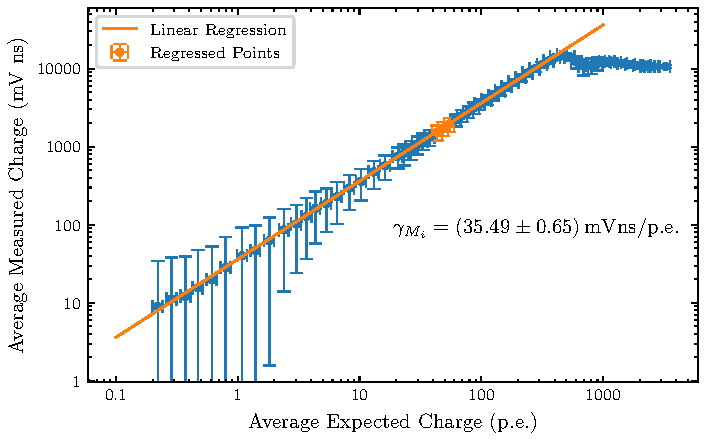
\includegraphics[width=\textwidth]{flat_fielding} 
	\caption[Flat-field calibration]{The average measured charge per illumination for a single pixel. The orange points were used for a linear regression through the origin in order to determine the flat-field coefficients for each pixel.} 
	\label{fig:flat_fielding}
\end{figure}

\begin{figure}
	\centering
    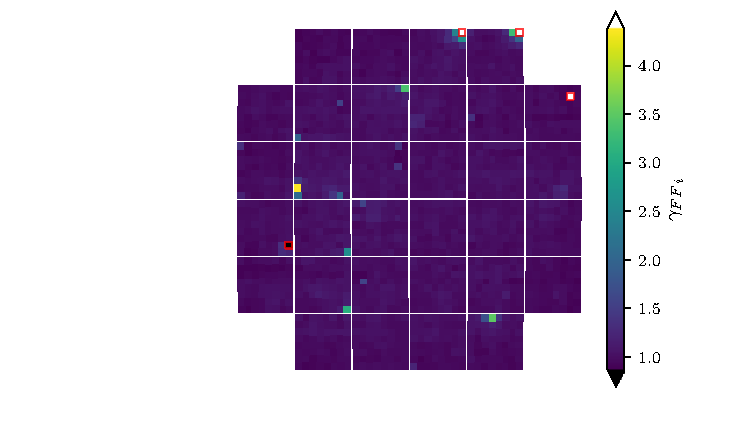
\includegraphics[width=\textwidth]{ff_values_cropped} 
	\caption[Flat-field Coefficients]{Camera image of the flat-field coefficient value, ${\gamma_{FF}}_i$, per pixel. Pixels that were designated ``dead'' or misbehaving are outlined in red, and exist beyond the colour-scale range.}
	\label{fig:ff_values}
\end{figure}

\begin{figure}
	\centering
    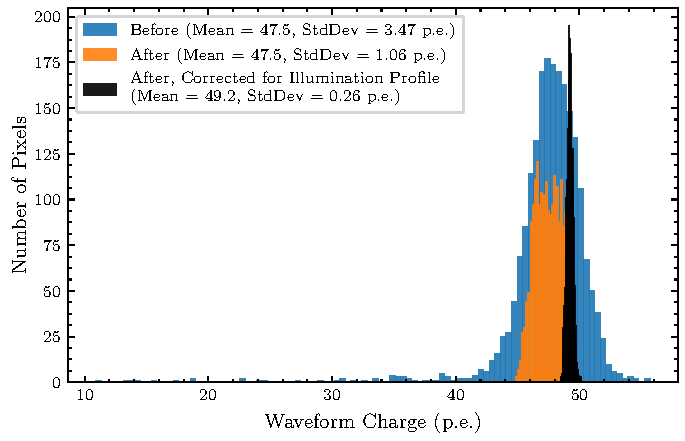
\includegraphics[width=\textwidth]{before_after_ff} 
	\caption[Flat-field Residuals]{Comparison between the spread in the average signal amplitude per pixel before (blue) and after (orange) the flat-fielding calibration. The charges were extracted from a dataset where a theoretical pixel located at the centre of the camera would be expected to have a charge of \SI{47.7}{\pe}. The black histogram contains the charges after the difference in the illumination profile (Section~\ref{section:illumination_profile}) between the pixels was considered, i.e. they contain the charge that would be measured if every pixel was located at the camera centre. Every pixel in the camera was included in the histograms.}
	\label{fig:before_after_ff}
\end{figure}

Once the ``expected charge'' dependence on filter-wheel position/transmission is characterised (Section~\ref{section:expected_charge}), we can calculate the coefficients, ${\gamma_M}_i$, required to convert the average extracted charge (in \si{mV ns}) into the charge we expect (in photoelectrons/photons). The application of these coefficients to the extracted charge has two effects:
\begin{itemize}
\item The signal response between pixels is homogenised - the same average amount of charge will be extracted for any pixel illuminated with an average of N photons.
\item The signal response is converted into the common telescope-array units of photoelectrons or photons.
\end{itemize}
Therefore:
\begin{equation} \label{eq:ff}
{\gamma_M}_i = \frac{\gamma_Q}{{\gamma_{FF}}_i}.
\end{equation}

To obtain ${\gamma_M}_i$ per pixel $i$ in the lab, datasets with around \SI{50}{\pe} expected charge per pixel were produced. For each pixel, the average extracted charge (in \si{mV ns}) was linearly regressed, while forcing the fit through the origin. This regression is shown for a single pixel in Figure~\ref{fig:flat_fielding}. The resulting gradient of the regression is equal to ${\gamma_M}_i$, which was combined with Equations~\ref{eq:photosensor_calibration}~\&~\ref{eq:ff} to obtain the calibrated extracted charge. The value of $\gamma_Q$ obtained for \gls{chec-s} was \SI{32.56}{mVns/\pe}\change{update with latest}, and the spread of $\gamma_{FF}$ across the camera is shown in Figure~\ref{fig:ff_values}. The resulting residual spread in signal response between pixels at an average camera illumination of \SI{47.7}{\pe} is shown in Figure~\ref{fig:before_after_ff}. The final variation in signal response between pixels at this illumination was 0.5\% \change{update when using the lab illumination profile}. The variation in signal responses at other illuminations is shown in Figure~\change{add figure}.

As the flat-field coefficients have been calculated in a manner in which they are unfolded from the illumination profile (by calculating the expected charge individually for each pixel), they are applicable to any environment the camera is used in. Any deviations that are observed in the signal between pixels are then due to the illumination profile present in the environment, and not due to the characteristics of the photosensor. Once the camera is on the telescope, the flat-field coefficients are intended to be routinely updated using the reflection of the LED flashers (Section~\ref{section:peripherals}) in the secondary mirror. This calibration will require an updated illumination profile in order to be performed.

\subsection{Dead Pixels}

Figure~\ref{fig:ff_values} shows that some of the photosensor pixels contained either no signal or an odd signal, resulting in an extreme flat-field coefficient. This was likely due to damage to the pixel during handling, or due to water ingress. However, the four pixels constitute to \SI{0.2}{\percent} of the camera, therefore the camera is still well within the \requirementref{B-TEL-1295 Pixel Availability} \gls{cta} requirement (Chapter~\ref{ch3-architecture}). These pixels were excluded from any calculations involving multiple pixels, including the expected-charge calibration and the camera charge-resolution. 

\section{Saturation Recovery}

\begin{figure}
	\centering
    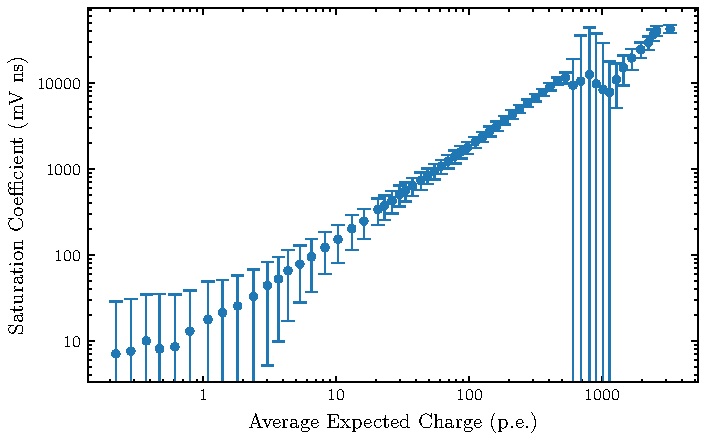
\includegraphics[width=\textwidth]{saturation_recovery} 
	\caption[Saturation Recovery.]{Initial investigation into recovering charge from a saturated waveform for the same pixel as shown in Figure~\ref{fig:flat_fielding}. The saturation coefficient is the integral from just before the pulse maximum, to the end of the waveform readout.}
	\label{fig:saturation_recovery}
\end{figure}

As evident in Figure~\ref{fig:flat_fielding}, high illumination (greater than \utilde\SI{200}{\pe}) measurements are affected by saturation of the detector. The saturation shown is due to the \gls{target} \gls{asic}, which saturates before the photosensor. However, while the height of the pulse increased no further, the excess charge caused the pulse to extend further (Figure~\ref{fig:generation_tc}). Therefore, it could be possible to perform a simple correction for the saturation recovery by utilising this waveform behaviour. A simple, initial investigation into saturation recovery is shown in Figure~\ref{fig:saturation_recovery}, where the waveform was integrated in a window that started just before the pulse maximum, and extended to the end of the waveform. This resulted in an extracted charge that continued to increase with illumination, apart from in the region immediately after saturation. More investigation is required for this calibration.

\section{Timing Corrections} \label{section:timing_corrections}

Due to the routing of the electronics in the front-end, the electrical signal path is slightly different per channel, causing a small difference in apparent arrival of the pulse in the waveform. The relative arrival time per pixel can be seen in Figure~\change{add camera image showing relative time}. 

Not only does this need to be taken into consideration when investigating the timing performance, it also can have a significant impact on the charge extraction performance. This is because the charge extraction approaches typically rely on other pixels (neighbouring or entire camera, see Chapter~\ref{ch6-reduction}) sharing a compatible pulse time. A charge extraction routine that incorrectly extracts the charge by \SI{1}{ns} can have the impact on the charge resolution shown in Figure~\change{show impact of an incorrect time extraction on charge resolution, maybe of just TM?}. Discussions are ongoing on how to best include the timing corrections in the charge extraction.

\section{Future}

During the long development of \gls{chec}, the calibration procedure has evolved significantly. Multiple iterations of the procedures have occurred to:
\begin{itemize}
	\item Accommodate the changes required in the upgrades of hardware (such as from \gls{target5} to \gls{targetc}).
	\item Simplify the calibration to save on computing resources.
	\item Account for additional factors, thereby improving the calibration (such as the \gls{ac} contribution to the Transfer Functions).
\end{itemize}
Therefore, while each iteration improves in one aspect, it may be at the expense of the others. As a result, the \gls{target} calibration procedure described in this chapter appears quite complicated compared to the approaches detailed by \textcite{Albert2017} and \textcite{Bechtol2012}. The next step in the calibration development for \gls{chec} is therefore to review the procedure used, with the aim of producing an approach that is simpler, includes aspects such as temperature dependence, and meets the requirements and processing rates required by \gls{cta}.
